\begin{problem}[9.]
    $r = \frac{2}{1 - \cos(\theta)}$
\end{problem}

\begin{solution}
    These problems are thankfully a lot more simple. Upon inspection we can see a few things. Firstly, we can tell that $e=1$ here which means we have a parabola. Nothing moves our focus, so that's at $(0,0)$. Since $e=1$ that means $d=2$ in this case. Due to that, our directrix is positioned at $x=-2$ making it a vertical line. Since our focus is to the right of the directrix our parabola will be opening to the right. Since the distance from the vertex to the focus is the same as the distance from the directrix to the vertex, our vertex must be positioned at $(-1,0)$, right smack dab in the middle of the two! Lastly we need the focal diameter. \bigskip
    
    The focal diameter is $4$ times the distance from the vertex to the focus. $4 \cdot 1 = 4$. Our focal radius then is 2. Based upon that information we can plot this bad boy. I'll be using desmos for simplicity but this explanation should indicate that I can do this manually as well.  
    
    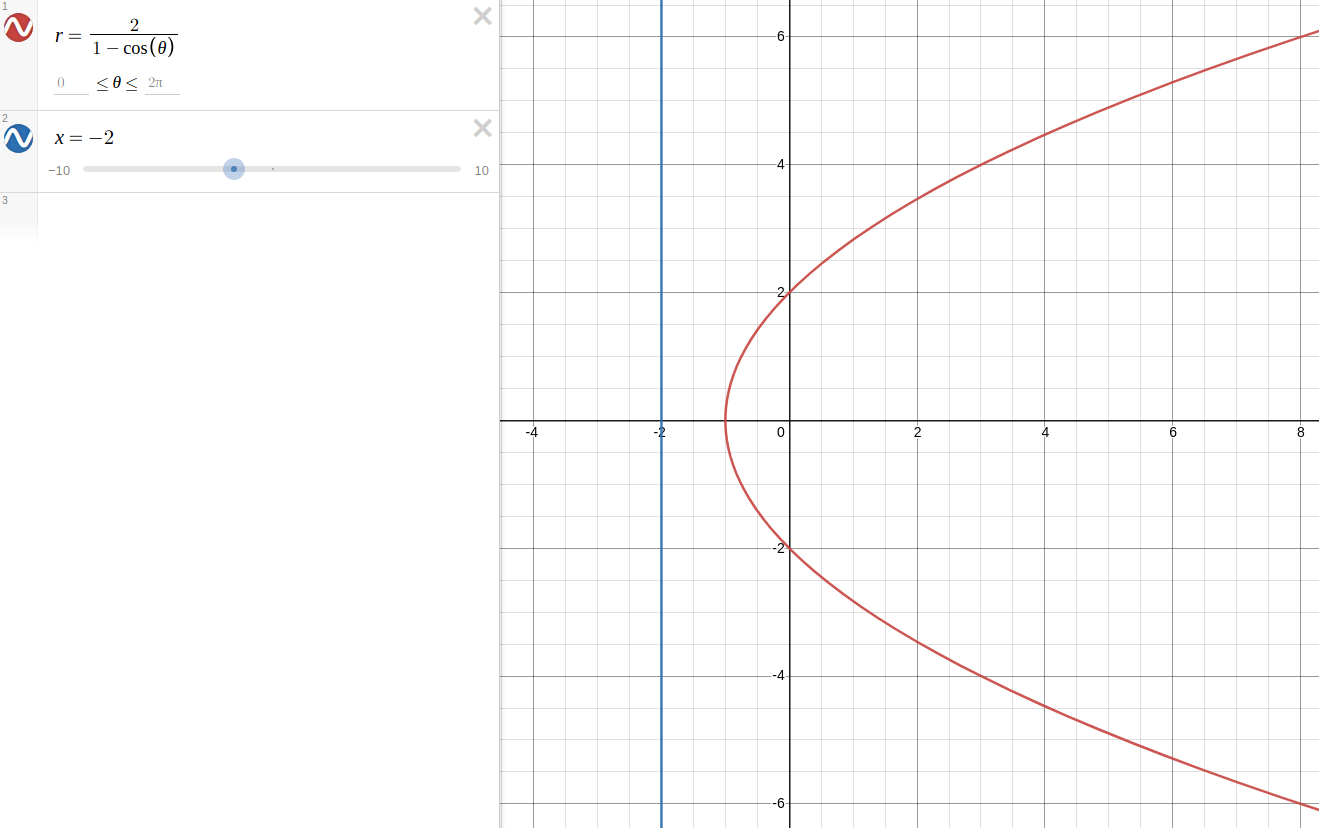
\includegraphics[scale = 0.3]{images/pr_9.png}
\end{solution}